\Chapter{ALGORITHMES D'OPTIMISATION SANS-DÉRIVÉES}\label{sec:Theme1}
\section{Coordinate Search}
Le premier algorithme à être abordé est aussi le plus intuitif pour l'optimisation sans contraintes, qu'on appelera \emph{Coordinate Search} (\CS{}), ou Recherche par coordonnée, parfois appelée \emph{Compass Search}~\cite{KoLeTo03a}. On attribue à Fermi et Metropolis~\cite{FeMe1952} cette première méthode de recherche directe. Pour que leur modèle suive bien leur ensemble de données expérimentales sur la diffusion nucléaire, Fermi et Metropolis ont fait varier les paramètre théoriques de déphasage de leur fonction un à la fois avec un pas constant. Lorsque ni l'augmentation ni la diminution de l'un des paramètres améliorait la concordance avec les données expérimentales, la longueur du pas était diminuée de moitiée et le processus était recommencé. On continuait ainsi jusqu'à ce que le pas soit considéré suffisement petit. C'est ainsi qu'est née la méthode de la recherche par coordonnée. 
Booker et al.~\cite{BoDeFrSeToTr99a} proposent un cadre rigoureux aux algorithmes de recherche de motifs. On y stipule que les algorithmes doivent être divisés en deux étapes, soient la recherche qu'on notera \SEARCH{} et la sonde qu'on notera \POLL{} afin d'être conforme avec la littérature. La \SEARCH{} consiste à l'implentation d'une méthode visant à explorer le domaine de la fonction sans égard à la détermination d'un optimum. Le \POLL{} cherche à minimiser la fonction pour déterminer un optimum. Dans le cadre qui nous intéresse, le \POLL{} serait l'entièreté du processus, tandis que la \SEARCH{} n'y trouverait pas son correspondant. La description de l'algorithme \CS{} décrite en vertu du cadre proposé par Booker et al. est fortement inspirée de celle de Audet et Hare, issue de~\cite{AuHa2018}.
\begin{algorithm}[H]
	\caption{\textsf{Recherche par coordonnée} (\CS)}
	\label{alg1}
	\begin{algorithmic}
		\STATE Avec $f:\R^n \rightarrowtail \R$ la fonction objectif et $x^0$ le point de départ
		\STATE 0. \textsf{Initialisation des paramètres} : 
		\bindent
		\STATE\begin{flushleft}
			\begin{tabular}{l l}
				$\delta^0 \in (0,\infty)$ & la longueur du pas initial\\
				$\epsilon_{\text{stop}} \in \left[ 0,\infty \right) $ & le critère d'arrêt\\
				$k \leftarrow 0$ & le compteur d'itérations\\
			\end{tabular}
		\end{flushleft}
		\eindent
		\STATE 1. \POLL
		\bindent
		\IF {$f(t) < f(x^k) $ pour un $t \in P^k := \{x^k \pm \delta^k e_i : i = 1,2,\dots,n \}$}
		\STATE $x^{k+1} \leftarrow t$ et $\delta^{k+1} \leftarrow \delta^k$
		\ELSE
		\STATE $x^{k+1} \leftarrow t$ et $\delta^{k} \leftarrow \frac{1}{2}\delta^k$
		\ENDIF
		\eindent
		\STATE 2. \textsf{Terminaison}
		\bindent
		\IF {$\delta^k \geq \epsilon_{\text{stop}}$}
		\STATE $k\leftarrow k+1$
		\STATE go to 1.
		\ELSE
		\STATE stop
		\ENDIF
		\eindent
	\end{algorithmic}
\end{algorithm}
À l'étape \POLL de l'algorithme, on entend que la fonction $f(x)$ est évaluée à chaque élément de $t \in P^k$ avant de déterminer quel $t$ deviendra le nouveau centre de sonde $x^{k+1}$. Cependant, si les évaluations sont effectuées en série, on aura une séquence de points à évaluer. La séquence proposée est celle de $2n$ mouvements dans les directions elementaires suivie de la détermination d'un nouveau centre de sonde si au moins une évaluation est un succès. C'est dans cette séquence que l'opportunisme pourra être introduit, afin de ne pas évaluer le reste de la liste si le test de décroissance simple est positif.
\section{Generalized Pattern Search}
Le deuxième algorithme présenté est la recherche par motifs généralisée. La premiere recherche par motifs en soit est élaboré par Hooke et Jeeves~\cite{HoJe61a}. Ils nomment la recherche par motifs (\emph{Pattern Search} ou \PS) la routine de recherche directe visant à minimiser une fonction $f(x)$ avec leur algorithme. Cette routine est composée d'une série de mouvements autour d'un point qui peuvent être divisés en deux types, soit les mouvements exploratoires (\emph{Exploratory Moves}) ou les mouvements destinés à la détermination d'un minimum, soit les mouvements de motifs (\emph{Pattern Moves}). Les mouvements exploratoires  servent à la détermination du motifs, c'est à dire au comportement de la fonction $f(x^k)$ aux alentours d'un point $x^k$. Les mouvements de motifs sont ensuite effectués dans la direction que les mouvements exploratoires ont déterminé comme étant celle qui se dirige vers le minimum de la fonction. Hooke et Jeeves introduisent aussi la définition de succès et d'échec. Un succès est mouvement tel que la valeur de $f(x)$ au point est inférieure à la meilleure connue auparavant. Dans le cas contraire, on dira que c'est un échec.\\
Lors de l'élaboration de cette technique ils mentionnent que :
\begin{quote}
	Par soucis de simplicité, les mouvements exploiratoires sont choisis de façon simple, c'est à dire, à chaque mouvement seulement la valeur d'une unique coordonée est changée.
\end{quote}
Pour ensuite affirmer que : 
\begin{quote}
	Suivant un mouvement de motif fructueux, il est raisonnable de conduire une série de mouvements exploratoires et de tenter d'améliorer d'avantage les résultats.
\end{quote}
De ces deux affirmations découlent les principes de bases de \PS{}, c'est à dire une sucscession de mouvements exploratoires dans les direction coordonnées $e_i : i =\pm \{1,2\dots n\}$ et d'un mouvement de motifs dans la meilleure direction. Chaque succès de la recherche de motifs entraine que la prochaine serie de mouvements exploratoires sera effectuée autour de ce nouveau meilleur point. Lorsque la succession échoue, la longueur du pas est réduite afin de déterminer un nouveau motif. Pour préciser la méthode, un point initial $x^0$ doit être déterminé ainsi qu'une longueur de pas initiale $\delta^0$ et un critère $\epsilon_{\textsf{stop}}$ pour lequel on jugera que le pas est devenu suffisement petit. De plus, on doit déterminer la méthode utilisée pour procéder à la réduction de la longueur du pas. Dans les mots de Hooke et Jeeves, le \POLL{} serait l'ensemble de mouvements exploratoires accompagné de la mise à jour du centre de sonde, tandis que la \SEARCH{} serait le mouvement de motif restant.\\
Torczon~\cite{Torc97a} amène une généralistation du \PS{} de Hooke et Jeeves. Dans cet article, l'auteure approche la méthode d'un autre oeil. Le motif propre à l'itération $P^k$ est issu de la multiplication de deux matrices $GC^k$, soient $G \in \R^{n\times n}$ la matrice de base et $C^k \in \R^{n\times p}, p > 2n$, la matrice generatrice. La matrice de base se doit d'être non-singulière et la matrice génératrice se doit d'être composée telle que $C^k = [\Gamma^k~ L^k]$, ou $\Gamma^k$ est la concaténation d'une matrice de plein rang $M$ et de son opposée. Le rôle de $\Gamma^k$ est de générer l'espace $\R ^n$, tandis que le rôle de la $L^k$ est de complémenter cette derniere avec des directions supplémentaires ne servant pas à strictement à générer l'espace, rappelant la \SEARCH{}. Ainsi, $GC^k$ est une matrice qui génére l'espace $\R^n$ et qui se libère du cadre restreignant des directions unitaires proposé par Fermi et Metropolis et repris par Hooke et Jeeves. Armés de $GC^k$ et d'une longueur de pas spécifique à une itération $\delta^k$, on retrouve $\delta^k Gc^k_i$, soit une généralisation de $\delta^k e_i$ présent dans \CS{}, mais pour lequel on a une colonne $c^k_i\in C^k$ perturbée par $G$ remplaçant la direction elementaire.\\
Toujours selon Torczon, la définition de mouvements exploratoires est reprises pour être plus générale. Un mouvement exploratoire est en fait un vecteur issu du motif $s^k \in P^k$. L'auteure demande aussi que, si il existe un vecteur colonne $c^k_i \in P^k$ tel que $f(x^k + \delta^k c_i^k) < f(x^k)$, alors les mouvements exploratoires doivent produire un pas $s^k$ tel que $f(x^k+s^k) < f(x^k)$.\\
L'algorithme s'inscrit alors en cinq étapes. Premièrement, à l'initialisation de l'algorithme, vient le calcul de la fonction $f(x)$ à l'itéré initial $x^0$ à l'itération $0$. Deuxièmement, le calcul d'une direction $s_k$ issue de la série de mouvements exploratoires. Troisièment, le calcul de $f(x^k + s^k)$. Ensuite vient la mise à jour $x^{k+1} = x^k +s^k$ si l'étape précédente est un succès, sinon $x^{k+1} = x^k$. Enfin, au besoin, on  met à jour l'ensemble générateur $C^k$ et la longueur du pas $\delta^k$ et on recommence le processus à partir de a deuxième étape jusqu'à ce que $\delta^k$ soit jugé suffisamment petit.\\
Afin de rester dans le cadre de Booker et al.~\cite{BoDeFrSeToTr99a}, on dépeint l'algoritme en se rattachant aux concepts de \POLL{} et de \SEARCH{}. Les directions issues de la matrice supplémentaire $f(x^k + s^k), s^k \in GL^k$ introduite par Torczon~\cite{Torc97a} correspondent à une étape de \SEARCH{} en vertu de sa fonction d'incorporer des directions supplémetaires à la recherche, tandis que les mouvements exploratoires visant à trouver un minimum autour du point de sonde ($f(x^k + s^k), s^k \in D\Gamma^k$) correspondent à la section \POLL{}. Cependant, on généralisera d'avantage $D\Gamma^k$ afin de le remplacer par un ensemble générateur positif~\cite{Davi54b}, noté $D=GZ, Z\in \R ^{n\times p}$, qui réponds aux exigence exactes énoncées dans~\cite{Torc97a} sans imposer que la taille de la matrice bornée supérieurement à $p = 2n$, mais bien tel que $n+1 \leq p \leq 2n$, en concordance avec les propriétés d'une base positive. Cette représentation est fortement inspirée de celle fournie par Audet et Hare dans~\cite{AuHa2018}. On dira de $S^k =GL^k$ qu'il est l'ensemble des directions supplémentaires $L^k$ fournit à l'itération $k$ soumit à une transformation par la matrice inversible  $G \in \R ^{n \times n}$.\\
Par ailleurs, il est à noter que les algorithmes de recherche directe énoncés dans~\cite{LeTo96b,Torc97a,LeTo99a,LeTo00a}, qui sont des algorithmes déclinant de la famille d'algorithmes \GPS, diffèrent à la formulation donnée dans ce document inspirée de Audet et Hare~\cite{AuHa2018}, notamment sur un aspect principal. La mise à jour de la longueur du pas se fait par deux paramètre différents, soient $\delta^{k+1} =\phi^k \delta^k, \phi^k \geq 1$ pour l'expansion du maillage dans le cas ou l'itération $k$ est un succès et $\delta^{k+1} =\lambda^k \delta^k, \lambda^k \in (0,1)$ dans le cas d'un échec. Dans la formulation présente on utilise un seul paramètre $\tau \in (0,1)$ et son inverse $\tau^{-1}$ pour cette mise à jour. Cependant, cette altération ne contrevient pas aux requis de la démonstration de la convergence de~\cite{Torc97a} qui assurent que la formulation présente possède les même propriétés. La formulation présente aussi une différence notable avec celle fait par Booker et al. dans~\cite{BoDeFrSeToTr99a}, c'est à dire l'admission de la mise à jour de la longueur du pas pour une \SEARCH fructueuse, alors que Booker et al. incorporent la mise à jour seulement dans un échec de \POLL, à l'image de l'utilisation d'un facteur $\phi^k=1$.
\begin{algorithm}[H]
	\caption{\textsf{Recherche par motifs généralisée} (\GPS)}
	\label{alg1}
	\begin{algorithmic}
		\STATE Avec $f:\R^n \rightarrowtail \R$ la fonction objectif et $x^0$ le point de départ
		\STATE 0. \textsf{Initialisation des paramètres} : 
		\bindent
		\STATE\begin{flushleft}
			\begin{tabular}{l l}
				$\delta^0 \in (0,\infty)$ & la longueur du pas initial\\
				$D=GZ$ & un ensemble générateur positif\\
				$\tau \in (0,1) \cup \Q$ & le paramètre d'ajustement du maillage\\
				$\epsilon_{\text{stop}} \in \left[ 0,\infty \right) $ & le critère d'arrêt\\
				$k \leftarrow 0$ & le compteur d'itérations\\
			\end{tabular}
		\end{flushleft}
		\eindent
		\STATE 1. \SEARCH
		\bindent
		\IF {$f(t) < f(x^k) $ pour un $t \in S^k$ } %\subseteq M^k$}
		\STATE $x^{k+1} \leftarrow t$ et $\delta^{k+1} \leftarrow \tau ^{-1}\delta^k$
		\STATE go to 3
		\ELSE
		\STATE go to 2.
		\ENDIF
		\eindent
		\STATE 2. \POLL
		\bindent
		\STATE détermination d'un ensemble générateur positif $\D^k \subseteq \D$
		\IF {$f(t) < f(x^k) $ pour un $t \in P^k := \{x^k + \delta^k d : d \in D^k\}$}
		\STATE $x^{k+1} \leftarrow t$ et $\delta^{k+1} \leftarrow \tau ^{-1}\delta^k$
		\ELSE
		\STATE $x^{k+1} \leftarrow t$ et $\delta^{k} \leftarrow \tau\delta^k$
		\ENDIF
		\eindent
		\STATE 3. \textsf{Terminaison}
		\bindent
		\IF {$\delta^k \geq \epsilon_{\text{stop}}$}
		\STATE $k\leftarrow k+1$
		\STATE go to 1.
		\ELSE
		\STATE stop
		\ENDIF
		\eindent
	\end{algorithmic}
\end{algorithm}
L'opportunisme pourra être implémenté dans l'étape de \POLL{} selon la même logique que dans \CS, c'est à dire à même la liste des points $x^k + \delta^k d : d \in D^k$. Pour ce qui est de la \SEARCH, l'implémentation de la stratégie est faisable mais sa performance n'en vient qu'à dépendre de la pertinence de la méthode pour générer $S^k$.
\section{Mesh Adaptive Direct Search}
Le troisième algorithme présenté est dans les même lignée que \CS et \GPS. Il s'agit de la recherche direct sur maillage adaptif (\emph{Mesh Adaptive Direct Search} ou \MADS), formulé par Audet et Dennis~\cite{AuDe2006}. Contrairement aux algorithmes précédents, \MADS est un algorithme basé sur un maillage, c'est à dire que chaque évaluation de la fonction objectif se fera à un point sur une discrétisation de l'espace des variables. On dénotera $M^k:=\{x^k + \delta^kDy : y \in \N^p\} \subset \R^n$ le maillage à l'itération $k$ sur lequel les itérés seront définis, généré par l'ensemble générateur positif $D = GZ$ et $y$ les entiers naturels. Il s'agit ici d'un maillage de cardinalité infini. Dans leur formulation de Audet et Hate reprise ici, les algorithmes \CS et \GPS sont aussi considéré comme étant basé sur un maillage, quoique leurs premières références~\cite{HoJe61a,Torc97a} n'en indique pas autant.\\
La grande distinction de \MADS ne réside alors pas dans son utilisation d'un maillage comme structure, mais bien l'incorporation d'un cadre à son étape de sonde. On définit le cadre tel que $F^k:=\{x\in M^k : \norminf{x-x^k} \leq \Delta^k b \}$ à l'itération $k$, soit l'ensemble des points sur le maillage $M^k$ pour lesquels la distance de Chebyshev à l'itéré courant est inférieur à une valeur $\Delta ^k b$. Cette valeur est déterminée par $b = \max\{\norminf{d'}:d' \in \D\}$, soit la plus grande composante vectorielle présente dans tous les colonnes de la base positive $\D$ issue de l'ensemble générateur $D$, multipliée par un paramètre introduit dans \MADS, soit le paramètre de longueur du cadre $\Delta^k$.\\
La figure \ref{fig:MADS} montre une itération hypothétique de \MADS pour laquelle $\Delta^k = \frac{1}{2}, \delta^k = \frac{1}{8}$ avec l'ensemble générateur étant
$D = \begin{bmatrix*}[C]
1 & 0 &-1\\
0 & 1 & -1
\end{bmatrix*}$. \\
\begin{figure}[H] %FIGURE  : MESH
	\begin{center}
		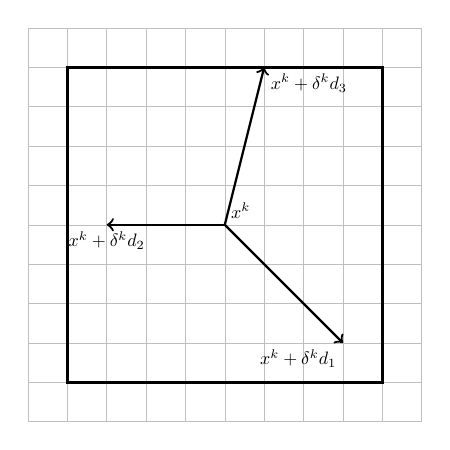
\begin{tikzpicture}
		% Flèches
		\draw [very thin,gray!50] (0,0) grid[step=0.5] (5,5);
		\draw [very thick] (0.5,0.5) rectangle (4.5,4.5);
		\draw [->,thick] (2.5,2.5)  -- (4,1) node [below left,scale=0.65]{$x^k+\delta^k d_1 $}; 
		\draw [->,thick] (2.5,2.5) -- (1,2.5) node [below,scale=0.65]{$x^k+\delta^k d_2 $};
		\draw [->,thick] (2.5,2.5) -- (3,4.5) node [below right,scale=0.65]{$x^k+\delta^k d_3 $};
		\draw (2.5,2.5) node [above right,scale=0.65]{$x^k$};
		\end{tikzpicture}
	\end{center}
	\caption{Ensemble générateur, maillage et cadre}
	\label{fig:MADS}
\end{figure}
Dans \GPS, quoique l'algorithme décrit n'inclue pas de maillage formellement, les évaluations sont limitées aux directions de $D$ mise à l'échelle avec la longueur du pas. Dans \MADS, on pourra choisir n'importe quelle direction telle que $x^k + \delta^k d$,tant que l'ensemble des directions $d$ forment un ensemble générateur positif $D_\Delta^k$ qui soit compris dans le cadre $F^k$. La mise à jour de la longueur du cadre se fait avec le paramètre d'ajustement du maillage qui, dans \CS et \GPS, servait  pour la mise à jour de $\delta^k$. Dans \MADS, $\delta^k$ est mis à jour par défaut est d'utiliser $\delta^k = \min(\Delta^k, (\Delta^k)^2)$. Ainsi, on s'assure de respecter $\delta^k \leq \Delta^k$ et on augmente exponentiellement le nombre de directions possibles si $\Delta^k \leq 0$. Afin de rester dans le cadre de Booker et al.~\cite{BoDeFrSeToTr99a}, on décrit l'algorithme en se rattachant aux concepts de \POLL et \SEARCH avec un étape \SEARCH limitée à un ensemble $S^k$ de points.  La description de l'algorithme est fortement inspirée de celle de Audet et Hare, issue de~\cite{AuHa2018}. 
\begin{algorithm}[H]
	\caption{\textsf{Recherche par treillis adaptifs} (\MADS)}
	\label{alg1}
	\begin{algorithmic}
		\STATE Avec $f:\R^n \rightarrowtail \R$ la fonction objectif et $x_0$ le point de départ
		\STATE 0. \textsf{Initialisation des paramètres} : 
		\bindent
		\STATE\begin{flushleft}
			\begin{tabular}{l l}
				$\Delta^0 \in (0,\infty)$ & la longueur du cadre initial\\
				$D=GZ$ & un matrice génératrice positive\\
				$\tau \in (0,1) \cup \Q$ & le paramètre d'ajustement du maillage\\
				$\epsilon_{\text{stop}} \in \left[ 0,\infty \right) $ & le critère d'arrêt\\
				$k \leftarrow 0$ & le compteur d'itérations\\
			\end{tabular}
		\end{flushleft}
		\eindent
		\STATE 1. \textsf{Mise à jour des paramètres}
		\bindent
		\STATE $\delta^k \leftarrow \min(\Delta^k,(\Delta^k)^2)$
		\eindent
		\STATE 2. \SEARCH
		\bindent
		\IF {$f(t) < f(x^k) $ pour un $t \in S^k$ } %\subseteq M^k$}
		\STATE $x^{k+1} \leftarrow t$ et $\Delta^{k+1} \leftarrow \tau ^{-1}\Delta^k$
		\STATE go to 4
		\ELSE
		\STATE go to 3
		\ENDIF
		\eindent
		\STATE 3. \POLL
		\bindent
		\STATE avec le cadre $F^k$ de demi-coté $\Delta^k$
		\STATE détermination d'un ensemble générateur positif $\D^k_\Delta \subset F^k$
		%\STATE tel qu'il est un sous-ensemble du cadre $F^k$ de demi-coté $\Delta^k$.
		\IF {$f(t) < f(x^k) $ pour un $t \in P^k := \{ x^k + \delta^k d : d \in \D ^k_\Delta\}$}
		\STATE $x^{k+1} \leftarrow t$ et $\delta^{k+1} \leftarrow \tau ^{-1}\Delta^k$
		\ELSE
		\STATE $x^{k+1} \leftarrow t$ et $\delta^{k} \leftarrow \tau\Delta^k$
		\ENDIF
		\eindent
		\STATE 4. \textsf{Terminaison}
		\bindent
		\IF {$\delta^k \geq \epsilon_{\text{stop}}$}
		\STATE $k\leftarrow k+1$
		\STATE go to 1.
		\ELSE
		\STATE stop
		\ENDIF
		\eindent
	\end{algorithmic}
\end{algorithm}
L'implémentation de la stratégie opportuniste sera faite à l'étape de \POLL selon la même logique que pour \CS et \GPS. 
\section{Generating Set Search}
Le quatrième algorithme est la recherche par ensemble générateur. Il est introduit par Kolda, Lewis et Torczon dans~\cite{KoLeTo03a} sous le nom de \textit{Generating Set Search} qu'on abrègera \GSS. Il s'agit d'un algorithme très similaire à \GPS mais qui incorpore certains aspects laissés de côté lors de la formulation de \GPS et certains aspects nouveaux propre à \GSS. À l'instar de \GSS, un ensemble de direction à chaque itération est dédié à la \SEARCH, soit $H^k$ et un ensemble dédié à la \POLL, soit $D^k$.

La différence principale entre \GSS et \GPS est le critère d'acceptation d'un itéré comme étant un succès. Pour les algorithmes précédents, chaque itération entrainant une simple diminution $f(x^k+\delta^kd)<f(x^k)$ était considérée comme un succès. Dans \GSS, on permet que le critère d'acceptation soit resserré avec l'addition du terme $\rho(\delta^k)$ au test de diminution, soit que $f(x^k+\delta^kd)<f(x^k)+\rho(\delta^k)$. $\rho(\delta)$ sera appelée la fonction de force et doit satisfaire à une des deux définitions. Soit $\rho(\delta)$ est continue, $\rho(\delta) = o(\delta)$ lorsque $\delta \downarrow 0$ et que $\rho(\delta_1) < \rho(\delta_2)$ si $\delta_1 < \delta_2$, ou soit $\rho(\delta)\equiv0$. Le premier cas impose une diminution suffisante de la fonction, rappelant le critère d'Armijo~\cite{Armi66a,griva2009linear}. Cet outil permet d'assurer la convergence globale théorique de l'algorithme en utilisant les résultats de convergence de Lucidi et Sciandrone~\cite{SLucidi_MSciandrone_2002} avec seulement une fonction objectif $f(x)$ bornée inférieurement. Le deuxième cas corresponds à une condition de diminution simple. Sous cette condition, les résultats de convergence globale sont assurés par les démonstrations faites sur les algorithmes basés sur treillis. Les conditions de convergences sont resserrés, de façon à ce que \GSS convergera dans le cas où les paramètres fournies restreignent les points candidats à un maillage, et qu'aucune expansion de ce maillage n'est admise.~\cite{KoLeTo03a,CoPr01a}. Il est à noter que \CS et \GPS sont des algorithmes de la famille de \GSS, c'est à dire qu'une paramétrisation spécifique de \GSS permets d'obtenir \GPS ou \CS.  
  
Les auteurs spécifient deux autres grande différences en comparaison avec \CS. Premièrement, on y fait valoir l'utilisation d'un ensemble générateur positif comme ensemble de directions de sonde, un aspect déjà incorporé dans notre définition de \GPS. L'autre différence se situe dans la souplesse des paramètres de contraction $\tau^k$ et des paramètres d'expansion $\phi^k$.\\
Plusieurs paramètres supplémentaires sont nécessaires tels que la mesure du cosinus, le plus petit angle entre deux directions de l'ensemble générateur $\kappa(G^k)$ qui empêche le choix de mauvaises directions, à l'instar de la mesure d'angle~\cite{griva2009linear,OrRh70a} en recherche linéaire. On y fait mention aussi de la longueur des vecteurs de l'ensemble générateur étant bornées tel que $\beta_{\min}<\norm{d}<\beta_{\max}, \beta_{\max} \geq \beta_{\min} >0$.
\begin{algorithm}[H]
	\caption{\textsf{Recherche par ensemble générateur} (\GSS)}
	\label{alg1}
	\begin{algorithmic}
		\STATE Avec $f:\R^n \rightarrowtail \R$ la fonction objectif et $x^0$ le point de départ
		\STATE 0. \textsf{Initialisation des paramètres} : 
		\bindent
		\STATE\begin{flushleft}
			\begin{tabular}{l l}
				$\delta^0 \in (0,\infty)$ & la longueur du pas initial\\
				$\lambda_{\max} \in (0,1) \cup \R$ & le paramètre de contraction maximale de la longueur du pas\\
				$\lambda^0{0} \in (0,1) \cup \R, \phi^0$ & les paramètre de contraction et d'expansion du pas\\
				\begin{tabular}{@{}l@{}}$\rho:[0,+\infty]\rightarrow\R$\\~
				\end{tabular} 
				&\begin{tabular}{@{}l@{}}une fonction continue tel que $\nabla(\rho(\delta)) < 0$ lorsque $\delta\rightarrow 0$\\
					et $\frac{\rho(\delta)}{\delta}\rightarrow 0$ quand $\delta \downarrow 0$\end{tabular} \\
				$\beta_{\max}\geq\beta_{\min}>0$ & les bornes sur la longueur des vecteurs de $G^k$\\
				$\epsilon_{\text{stop}} \in \left[ 0,\infty \right) $ & le critère d'arrêt\\
				$\kappa_{\min} \geq 0$ & La mesure cosinus minimale d'un ensemble\\
				$k \leftarrow 0$ & le compteur d'itérations\\
			\end{tabular}
		\end{flushleft}
		\eindent
		\STATE 1. \SEARCH
		\bindent
		\STATE détermination de $H^k = \{s \in \R^n,~\beta_{\min}\leq \norm{s}\}$
		\IF {$f(t) < f(x^k) - \rho(\delta^k) $ pour un $t \in S^k=\{x^k+\delta^ks, s \in H^k\}$ } %\subseteq M^k$}
		\STATE $x^{k+1} \leftarrow t$ et $\delta^{k+1} \leftarrow \phi^k \delta^k$
		\STATE go to 3
		\ELSE
		\STATE go to 2.
		\ENDIF
		\eindent
		\STATE 2. \POLL
		\bindent
		\STATE détermination de $D^k = \{s\in\R^n,~\beta_{\min}\leq\norm{s}\leq\beta_{\max},~\kappa(H^k\cup D^k)\geq \kappa_{\min}\} $
		\STATE un ensemble générateur
		\IF {$f(t) < f(x^k) $ pour un $t \in P^k := \{x^k + \delta^k d : d \in D^k\}$}
		\STATE $x^{k+1} \leftarrow t$ et $\delta^{k+1} \leftarrow \phi^k\delta^k$
		\ELSE
		\STATE $x^{k+1} \leftarrow t$ et $\delta^{k} \leftarrow \tau^k\delta^k$
		\ENDIF
		\eindent
		\STATE 3. \textsf{Terminaison}
		\bindent
		\IF {$\delta^k \geq \epsilon_{\text{stop}}$}
		\STATE $k\leftarrow k+1$
		\STATE go to 1.
		\ELSE
		\STATE stop
		\ENDIF
		\eindent
	\end{algorithmic}
\end{algorithm}
\section{Implicit Filtering}
Le dernier algorithme est celui du filtrage implicite (\textit{Implicit Filtering} ou \textsf{imfil}), une méthode développée par Kelley~\cite{Kell99b,Kelley2011}. \imfil se veut un algorithme d'optimisation sans-contraintes explicites hybride de recherche linéaire se basant sur le gradient simplex incorporant des particularités de \CS. On définira le gradient simplex de \imfil comme l'approximation du gradient en calculant la valeur de la fonction à chaque point d'un simplexe où il est possible de le faire.
\begin{gather*}
\nabla_{s}f(x^k) = \frac{1}{h^k}\delta(f,x^k,V,h)V^{\dagger}
\end{gather*}
avec $h$ le pas $V\in\R^{n \times k}$ une matrice représentant les directions du simplexe, $\delta(F,x,V,h^k)$ la matrice ayant $f(x+hv_j^1) - f(x)$ à sa $j^e$ colonne, $\{v_1^j\} \in V$ et $V^{\dagger}$ son inverse de Moore-Penrose~\cite{GoVL1996} et $h^k$ le pas de l'itération. L'utilisation de la pseudo-inverse est justifiée par la nécessité de calculer des différences finies d'un seul côté si un point du simplexe n'est pas réalisable. L'idée fondamentale de \imfil est de calculer le gradient simplex en un itéré courant $x^k$, avec des différences simples ou centrées, et d'utiliser ce gradient $\nabla_{s}f(x^k) \in \R^n$ comme direction pour effectuer une recherche linéaire à l'image d'une descente du gradient~\cite{NoWr2006}.  
  
L'algorithme est défini comme sans-dérivées puisqu'il n'utilise pas le calcul de dérivées analytiques de la fonction. Cependant, contrairement aux étapes de \POLL des algorithmes présentés précédemment, l'algorithme approxime la dérivée à l'aide de différences finies. Pour déterminer les valeurs de $f(x+hv_i^1)$ servant au calcul du gradient simplex, l'auteur introduit une nomenclature proche de la notre, soit le \textsf{stencil poll}, qu'on généralisera sonde du simplexe, qui est constituée de $n$ à $2n$ évaluations de la boîte noire, dans les cas opposés où deux contraintes de bornes sont actives et aucune contrainte de borne n'est active, si le motif utilisé est une combinaison des vecteurs unitaires de $\R^n$. C'est cette sonde du simplexe qui sera analogue aux sections \POLL des algorithmes présentés antérieurement.

Suivant la sonde du simplexe, si la celle-ci est fructueuse et que la norme de l'approximation du gradient simplexe n'est pas plus petite que $\tau h^k$, l'algorithme effectue une recherche linéaire dans la direction inverse du gradient simplexe $ d = -\nabla_{s}f(x^k)$ avec un nombre de de pas maximal spécifié par l'utilisateur. Alternativement, la direction peut-être calculée avec la résolution de $Hd = \nabla_{s}f(x^k)f(x^k)$, où $H \in \R^{n\times n}$ est une matrice Hessienne issue d'un modèle mis à jour selon une méthode de Quasi-Newton (par exemple Broyden-Fletcher-Goldfarb-Shanno (BFGS)~\cite{Broy65a,Flet65a}),$\nabla_{s}f(x^k) \in \R^n$ le gradient simplexe et $f(x^k)$ la fonction objectif évaluée à l'itéré courant. La recherche linéaire peut s'écrire de la façon suivante qu'on abrègera \textsf{BLS} pour \textit{Backtracking Line Search}. 
\begin{gather}
\underset{m}{\min}\{m~:~f(x^k-\beta^m d) < f(x^k),m \in \{0,\text{maxitarm}\}\cup\N\}.
\end{gather}
où $\beta^m\leq 1$ agit comme un facteur diminuant pour déterminer la longueur du pas nécessaire, $d \in \R^n$ la direction de descente, $m$ un entier servant de puissance à $\beta$ et  $\text{maxitarm}$ est le nombre maximal de pas de recherche linéaire imposé par l'utilisateur. L'idée ici est de trouver un $m$ minimal pour lequel la fonction évaluée en $f(x^k+\beta^m)<f(x^k)$.\\
Dans le cas ou la sonde échoue, la longueur du pas est diminuée de moitié et aucune autre recherche n'a lieu. L'algorithme est ainsi recommencé jusqu'à ce que la longueur du pas soit diminuée en deçà d'un seuil paramétré. La description de l'algorithme simplifié sort du cadre de travail précédemment imposé~\cite{BoDeFrSeToTr99a}, quoique l'algorithme pourrait être écrit de façon à avoir un \POLL suivi d'une \SEARCH conditionnelle au succès du \POLL.\\
\begin{algorithm}[H]
	\caption{\textsf{Filtrage implicite} (\imfil)}
	\label{alg5}
	\begin{algorithmic}
		\STATE Avec $f:\R^n \rightarrowtail \R$ la fonction objectif et $x^0$ le point de départ
		\STATE 0. \textsf{Initialisation des paramètres} :
		\bindent 
		\STATE\begin{flushleft}
			\begin{tabular}{l l}
				$h^0 \in (0,\infty)$ & la longueur du pas initial\\
				$V = \{\pm e_1,\pm e_2,\dots,\pm e_k\}$ & une matrice de motif\\
				$\text{budget}$ & le nombre d'évaluation maximal\\
				$\text{maxitarm}$ & nombre maximale d'itération de recherche linéaire\\
				$\epsilon_{\text{stop}} $ & le critère d'arrêt sur le pas\\
				$k \leftarrow 0$ & le compteur d'itérations de l'algorithme\\
				$\tau \leftarrow 0$ & la tolérance admise sur le gradient\\
			\end{tabular}
		\end{flushleft}
		\eindent
		\STATE 1. \textsf{Boucle principale} :
		\bindent 
		\WHILE {$f_{\text{count}} < \textsf{budget} ~\&~ h^k < \epsilon_{\text{stop}}$} %\subseteq M^k$}
%		\WHILE{$\norm{x^k-P(x^k-\nabla_{s}(x^k))}\geq \tau h$}
		\STATE Effectuer la sonde du gradient
		\FOR {$i=1,\dots,k$}
		\STATE $F_i = f(x^k + h^k v_i), v \in V$
		\ENDFOR
		\STATE Mise à jour de $H$ si nécessaire
		\STATE évaluer $-\nabla_{s}f(x^k)$    (ou $d = H^{-1}\nabla_{s}f(x^k)f(x^k)$)
		\STATE $x_{\min}\leftarrow\text{argmin}(F)$
		\IF {$\norm{\nabla_{s}f(x^k)}\geq \tau h^k$ \& $f(x_{\min})<f(x^k)$}
		\STATE $d \leftarrow -\nabla_{s}f(x^k)$
		\IF {\textsf{BLS} est réalisable}
		\STATE $ x^{k+1} \leftarrow x^k + \beta^m d$ 
		\ELSE
		\STATE $x^{k+1} \leftarrow x_{\min}$
		\ENDIF
		\ELSE
		\STATE $h^{k+1} \leftarrow {h^k}/{2}$
		\ENDIF
		\ENDWHILE
		\eindent
	\end{algorithmic}
\end{algorithm}
\section{Gestion des contraintes en DFO}
Le problème (1) demande que $x$ soit compris dans l'ensemble $\Omega$. On peut représenter $\Omega$ de la façon suivante afin de représenter le cas ou les seules contraintes existantes sont des bornes notées $X$.
\begin{gather*}
\Omega = X = \{x\ \in\ \R^n\ :\ l_i \leq (x)_i \leq u_i\}\\
\end{gather*}
Où $l \in \R^*\cup\{-\infty\}$ représente le vecteur des bornes inférieures et $u \in \R^*\cup\{+\infty\}$ le vecteur des bornes supérieures. Sous cette même forme, on peut définir un problème comme étant non borné, si toutes les valeurs de $l$ et de $u$ prennent la valeur infinie, ce qui équivaut à $ X = \R ^n$ \\
Si la variable $x$, en plus d'être limitée par des bornes, est contrainte par un ensemble d'inégalité, tel que : 
\begin{equation*}
\begin{aligned}
\underset{x\in X \subset \R ^n}{\min}& & & f(x)\\
\text{s.t.}& & & c(x) \leq 0\\
\end{aligned}
\end{equation*}
On peut représenter son ensemble $\Omega$ réalisable tel que
\begin{gather*}
\Omega = \{x~\in~X~\subset \R ^n~:~ c(x) \leq 0\}
\end{gather*}
où $c:x\rightarrow \R ^n$. Une approche pour traiter ce problème se nomme \textbf{la barrière extrême}~\cite{AuDe2006}. On définit une fonction de barrière suivante
\begin{align*}
f_\Omega = \begin{cases}
f(x)~ &\text{si $x \in \Omega$}\\
\infty~ &\text{sinon}
\end{cases}
\end{align*}
On peut alors redéfinir la fonction à optimiser comme étant $f_\Omega$ en ne se souciant plus des contraintes. Cependant, dépendemment de la forme de la boîte noire, il est possible qu'une solution $f(x)$ existe, et ce même si l'évaluation de $c(x)<0$. On peut alors quantifier la violation de contrainte ainsi~\cite{AuHa2018} : 
\begin{align*}
h(x) = \begin{cases}
\sum_{j\in J}^{}(\max(c_j(x),0))^2~ &\text{si}~x\in X\\
\infty~ &\text{sinon}
\end{cases}
\end{align*}
Avec $J$ l'ensemble des indices des contraintes et $X$ l'ensemble des points. Ces contraintes seraient alors relaxables. Audet et Dennis~\cite{AuDe09a} proposent une façon de gérer la relaxation avec la \textbf{barrière progressive}. Afin de déterminer une hiérarchie des points selon leur valeur de $h(x)$ et $f(x)$, on définie des notions de dominance entre deux points. On dit que le point $x$ réalisable domine le point $y$ réalisable si l'expression suivante est respectée 
\begin{align*}
f(x) < f(y) \implies x\prec_{f} y ~ &\text{si}~x,y\in\Omega.\\
\end{align*}
Cependant, si $x$ est non-réalisable, il domine le point $y$ non-réalisable si
\begin{align*}
f(x) \leq f(y), h(x)\leq h(y) \implies x\prec_{h} y ~ &\text{si}~x,y\in\Omega/X
\end{align*}
avec au moins une inégalité stricte.\\
L'algorithme de la barrière progressive admet deux solutions courantes, soient $x^{feas}$ la solution réalisable dont la valeur de la fonction objectif est minimale, et $x^{inf}$, la solution irréalisable non-dominée dont la valeur de la fonction objectif est minimale et où $h(x^{feas})$ est inférieur à $h^k_{max}$, un paramètre limite pour $h$ spécifique à l'itération $k$.\\
\\
Dans la Figure ~\ref{fig:barrier}, on observe peut voir quelques points candidats. Les points pleins sont les points non-dominés et les points vides sont dominés ou exclus par la barrière $h_{max}$. Ceux présent dans la zone grise sont dominés par des points irréalisables pour lesquels $f(x)$ ou $h(x)$ sont inférieurs,  ou encore leur valeur de leur fonction de violation $h(x)$ est supérieur à $h_{max}$. L'interaction entre l'utilisation des concepts de barrière et les différents algorithmes d'optimisation sans dérivées sera vue lors de la description des algorithmes.
\begin{figure}[h]
	\begin{center}
		\begin{tikzpicture}
		% Flèches
		\draw[->] (0,0) -- (8,0);
		\draw [->] (0,0) -- (0,5);
		% Axes 
		\draw (8,0) node[right] {$h$};
		\draw (0,5) node[above] {$f$};
		% Point faisable non domin
		\draw (0,3.5) node[]{$\bullet$};
		\draw (0,3.5) node[below left]{$x^{feas}$};
		%Point faisable dominé
		\draw (0,4.5) node[]{$\circ$};
		% Points non-dominés mais pas inf
		\draw (2,3.9) node[]{$\bullet$};
		\draw (4,1.7) node[]{$\bullet$};
		% Point non-dominé inf
		\draw (6,0.7) node[]{$\bullet$};
		\draw (6,0.7) node[below left]{$x^{inf}$};
		% Points dominés
		\draw (2.9,4.2) node[]{$\circ$};
		\draw (5,1.7) node[]{$\circ$};
		\draw (6.6,1) node[]{$\circ$};
		\draw (7.5,0.5) node[]{$\circ$};
		% Droites delimitant zone realisable
		\draw [-] (2,5) -- (2,3.9);
		\draw [-] (2,3.9) -- (4,3.9);
		\draw [-] (4,3.9) -- (4,1.7);
		\draw [-] (4,1.7) -- (6,1.7);
		\draw [-] (6,1.7) -- (6,0.7);
		\draw [-] (6,0.7) -- (7,0.7);
		% Droite pour h max
		\draw [-] (7,0) -- (7,5);
		\draw (7,0) node[below]{$h_{max}$};
		% Hachure de la région dominée
		\fill[pattern = north east lines,opacity = 0.5] (2,5) -- (2,3.9) -- (4,3.9) -- (4,1.7) -- (6,1.7) -- (6,0.7) -- (7,0.7) -- (7,0) -- (8,0) --(8,5) -- cycle;
		\end{tikzpicture}
	\end{center}
	\caption{Barrière progressive, dominance et solutions courantes multiples} \label{fig:barrier}
\end{figure}
